% Poner en perception (sonido, luz). ??

\title{Visual Redundancy}

\maketitle
\tableofcontents

Usually, some part of the data in an image is
\href{https://en.wikipedia.org/wiki/Data_redundancy}{redundant} (can
be removed without loss of information).

\section{Statistical redundancy}
\href{https://en.wikipedia.org/wiki/Redundancy_(information_theory)}{Statistical
  redundancy} is present in all those sequences of symbols where we
can infeer a probability of ocurrence of a symbol taking into
consideration the rest of symbols of a sequence. Statistical redudancy
can be found in text, audio, image and video, among other types of
signals.

Statistical redundancy can be removed by text compressors.

Statistical redundancy is also called source-coding redundancy~\cite{kondoz2009visual}.

\section{Temporal}
Temporal redundancy is shown by sequences of samples when those
samples are similar in value and when paterns of samples tend to
repeat. Temporal redundancy is found in all those time-dependant
signals, such as
\href{https://en.wikipedia.org/wiki/Inter_frame}{audio} and
\href{https://en.wikipedia.org/wiki/Inter_frame}{video}, among others.

Temporal redundancy can be removed by most audio and video codecs.

Most video codecs use motion compensation to remove temporal redundancy.

\section{Spatial (2D)}
\href{https://robbfoxx.wordpress.com/2015/07/12/discussion-6-2-1-what-is-redundancy-temporal-redundancy-and-spatial-redundancy/}{Spatial
  redundancy} is present basically in images, because pixels tend to
be similar to their neighbors or tend to repeat textures. See
Fig~\ref{fig:correlacion_lena}.

\begin{figure}
  %\pngfig{graphics/correlacion_lena}{8cm}{800} %
  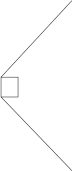
\includegraphics{graphics/correlacion_lena}
  \caption{Spatial redundancy in images.}
  \label{fig:correlacion_lena}
\end{figure}

Humans are more sensitive to low-frequency image data than
high-frequency data. In addition, luminance information is more
important than chrominance information~\cite{kondoz2009visual}.

\section{Color ($\text{RGB}$)}
In $\text{RGB}$ images, the color of a pixel depends on the
\href{https://en.wikipedia.org/wiki/Visible_spectrum}{frequency of the
  light that the pixel represents}. Such information can be
represented in a number of different encoding systems known as
\href{https://en.wikipedia.org/wiki/Color_space}{color spaces}. Among
all those systems, the $\text{RGB}$ color space is the most used
because $\text{RGB}$ images can be obtained directly from the light
signal using color filters.\footnote{Specifically, a red (R) filter, a
green (G) filter and a blue (B) filter.}

The $\text{RGB}$ color model has evident physical advantages and it is
straightforward and easy to manage, but also, in general, is quite
\href{https://en.wikipedia.org/wiki/Data_redundancy}{redundant}. In
the case of a $\text{RGB}$ image, the three components of each pixel
are usually highly
\href{https://en.wikipedia.org/wiki/Correlation_and_dependence}{correlated}
in the sense that, for example, if the $\text{R}$ component of a pixel
has a high value, the other components will be also high, with a high
probability. This means that if we use an encoding system that takes
into consideration this redundancy, we can express the same
information\footnote{Or almost the same amount of information,
depending on the accuracy of the computations.} using a smaller number
of bits (reducing thus the length of the code-stream).

\begin{figure}
  \centering
  %\png{san-diego_chroma_subsampled}{1000}
  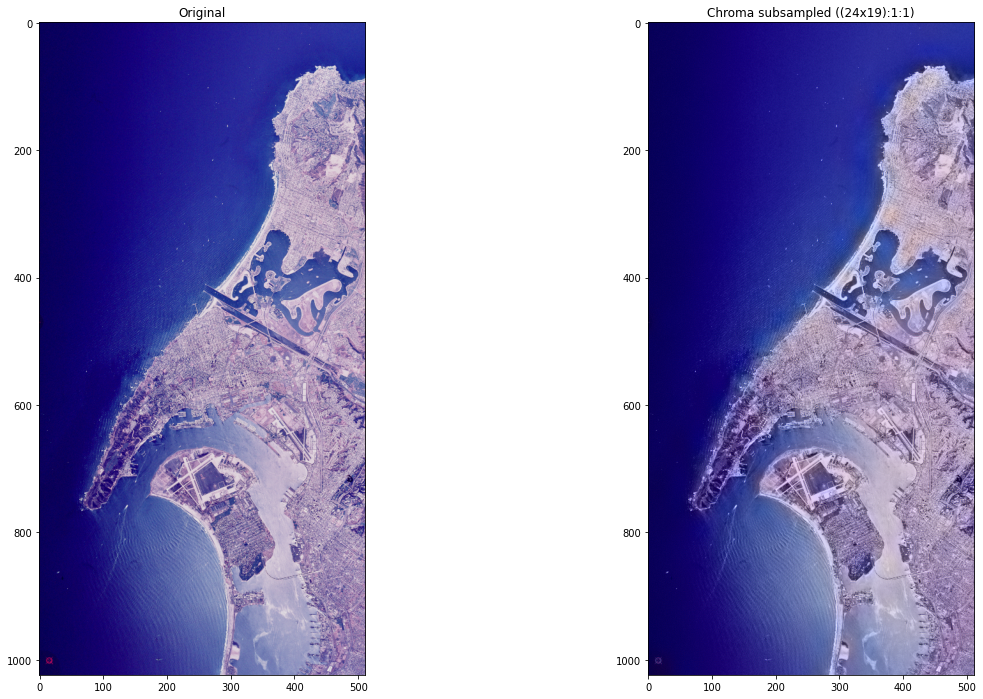
\includegraphics{san-diego_chroma_subsampled}
  \caption{Effect (visual) of chroma subsamplig in the $\text{YCrCb}$ domain. See
    this
    \href{https://github.com/vicente-gonzalez-ruiz/visual_redundancy/blob/master/chroma_subsampling.ipynb}{notebook}.}
  \label{fig:san-diego_chroma_subsampled}
\end{figure}

Visual color redundancy (generated by the way that humans perceive the
chrominance) is exploited by most color models used in image and video
compression, such as $\text{YCrCb}$ and $\text{YCoCg}$. This can be
see in the Fig.~\ref{fig:san-diego_chroma_subsampled}.

\section{Measurement of the redundancy}
\href{https://en.wikipedia.org/wiki/Redundancy_(information_theory)}{redundancy}
we have basically two options:
\begin{enumerate}
\item Compute the
  \href{https://en.wikipedia.org/wiki/Entropy_(information_theory)}{0-order
    (memoryless source) entropy} of the signal: the higher the
  entropy, the lower the redudancy. In fact, if we suppose that the
  samples of the signal are uncorrelated, the 0-order entropy is an
  exact measure of the expected bit-rate achieved by an
  \href{https://en.wikipedia.org/wiki/Arithmetic_coding}{arithmetic
    encoder} (the most efficient entropy compressor). Unfortunately,
  the 0-order entropy is usually only a estimation of the redundancy,
  i.e., lower bit-rates can be achieved in practice after using a high-order
  decorrelation.
\item A better way is to use an
  \href{https://en.wikipedia.org/wiki/Data_compression}{lossless
    compressor}: the higher the length of the compressed file compared
  to the length of the original file, the lower the
  redundancy.\footnote{If the length of the compressed file is equal or
  larger than the length of the original file, then, for the compressor
  that we are using, there is not redundancy in the original
  representation.} Notice, however, that although this estimation is
  more accurate than the 0-order entropy, in general, it depends on the
  compressor (different algoritms can provide different
  estimations).
\end{enumerate}


\section{Resources}
\renewcommand{\addcontentsline}[3]{}% Remove functionality of \addcontentsline
\bibliography{maths,data-compression,signal-processing,DWT,image-compression,image-processing}
